In diesem Kapitel werden erste Entwürfe der Benutzeroberflächen dargestellt. Dabei sind weder die ästhetischen Aspekte noch die Anordnung der Inhalte in ihrer finalen Version.

\begin{figure}[h]
	\centering

	\begin{tabularx}{\textwidth}{ p{.5\textwidth} | X }
		\textbf{Skizze} & \textbf{Beschreibung}

		\\ \hline \\

		\raisebox{-.9\height}[0pt][0pt]{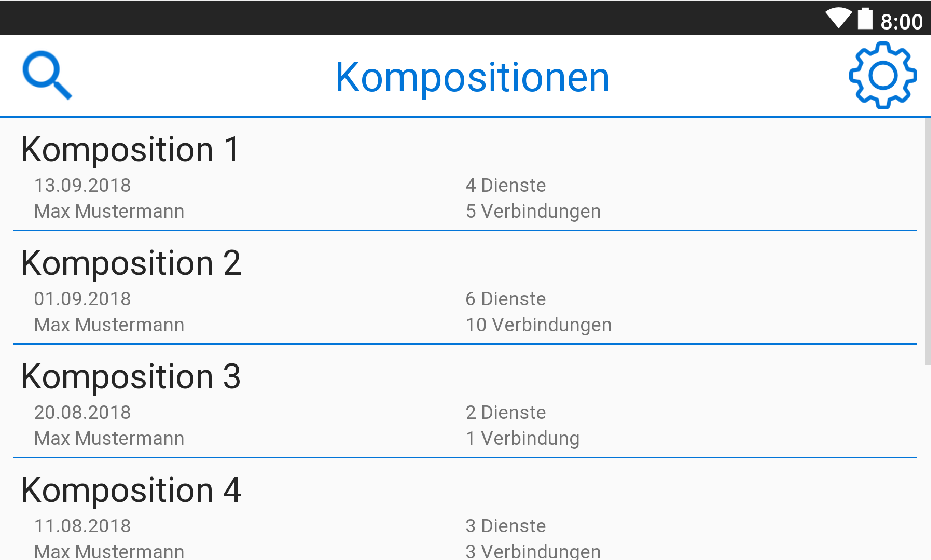
\includegraphics[width=.5\textwidth]{img/mockup_list}}
		%\caption{Listenansicht in der Android-App}
		\label{fig:mock-list}

		&In der Listenansicht werden dem Nutzer alle für ihn sichtbaren Kompositionen mit einigen Informationen (Ersteller, Erstellungsdatum, ...) angezeigt. Falls er nicht eingeloggt ist, sieht er nur die öffentlichen Kompositionen. Durch ein Tippen auf das Lupen-Symbol besteht die Möglichkeit, die Liste zu filtern. Durch das Antippen des Zahnrad-Symbols gelangt der Nutzer in ein Menü, in dem er sich unter anderem ein- und ausloggen kann.

		\\ \hline \\
		\raisebox{-.9\height}[0pt][0pt]{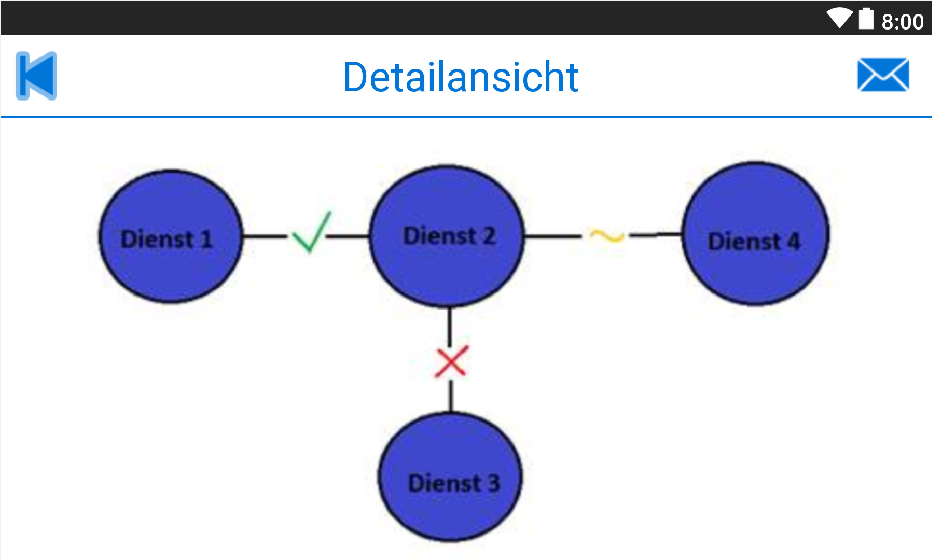
\includegraphics[width=.5\textwidth]{img/mockup_detail}}
		%\caption{Detailansicht in der Android-App}
		\label{fig:mock-detail}

		&
		Durch das Antippen einer Komposition aus der Listenansicht wird die Detailansicht geöffnet. Hier wird die Komposition als Graph dargestellt. (Fehlende) Kompatibilität wird an den Verbindungen gekennzeichnet. Mit dem Brief-Symbol kann die angezeigte Komposition verschickt werden.  Dabei wird ein PDF erstellt, das sowohl den Graphen als auch einige Details in textueller Form enthält.

	\end{tabularx}

	\caption{Mockup der Android-App}
	\label{fig:app-mockup}
\end{figure}


\begin{figure}[h]
	\centering
	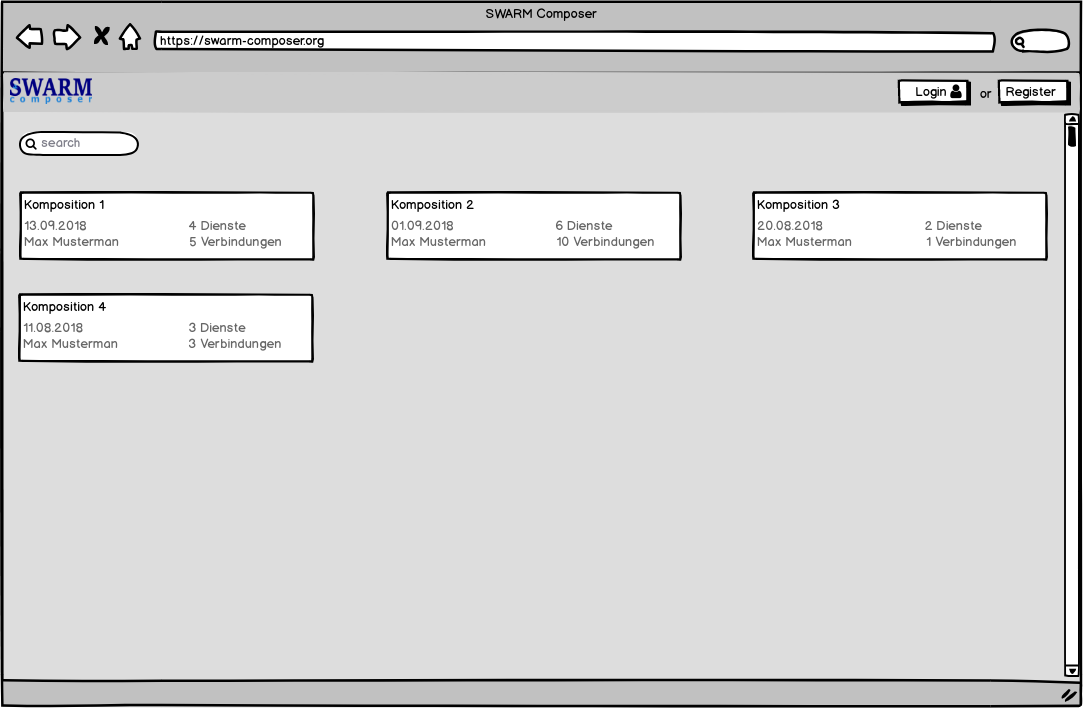
\includegraphics[width=\textwidth]{img/kompositionen}
	\caption{
            Dies ist die konzipierte Startseite. Nicht eingeloggte Nutzende bekommen alle
            öffentlich einsehbaren Kompositionen angezeigt. Durch das Drücken
            auf eine Komposition wird der Nutzende zur Bearbeitungsseite weitergeleitet.
        }
	\label{fig:kompositionen}
\end{figure}

\begin{figure}[h]
	\centering
	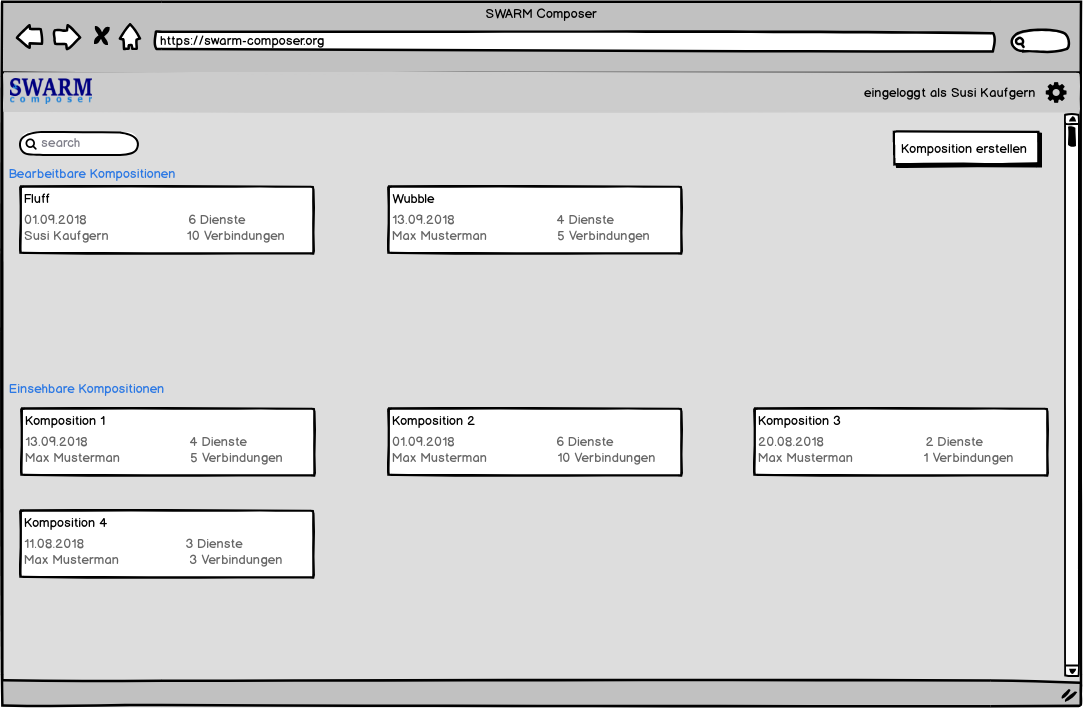
\includegraphics[width=\textwidth]{img/kompositionen_eingeloggt}
	\caption{
          Eingeloggte Nutzende können zusätzlich zu den ihnen sichtbaren Kompositionen
          auch noch für sie bearbeitbare Kompositionen getrennt sehen.
        }
	\label{fig:kompositionen-eingeloggt}
\end{figure}

\begin{figure}[h]
	\centering
	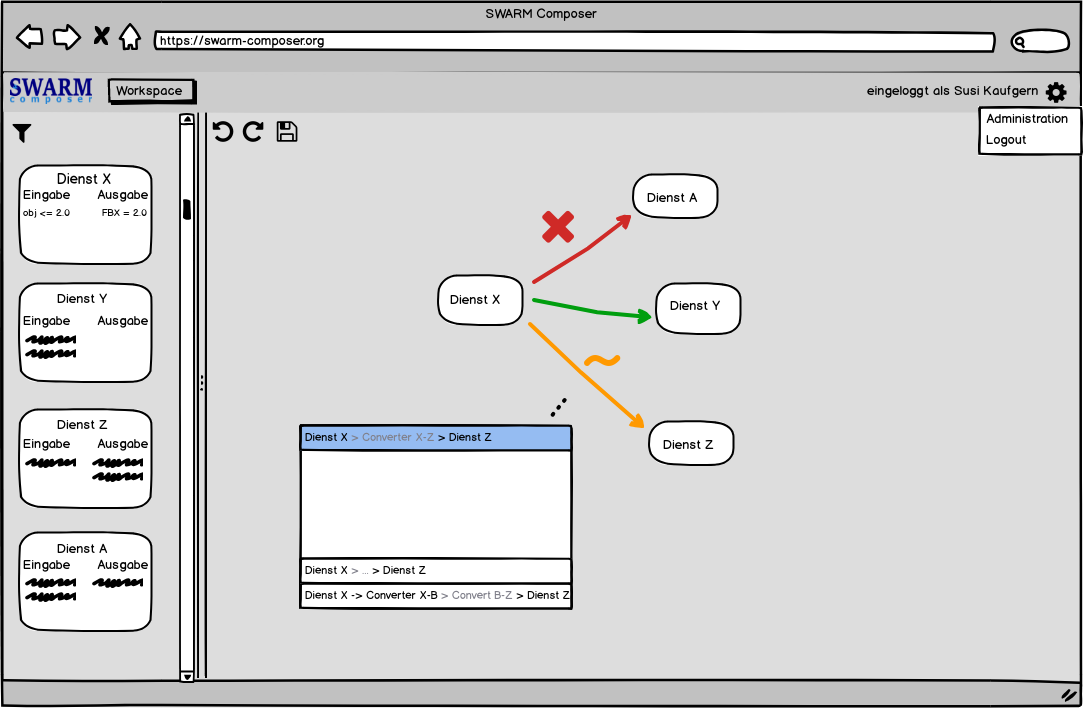
\includegraphics[width=\textwidth]{img/editor}
	\caption{
            Hier können eingeloggte Nutzende eine zuvor gewählte Komposition
            bearbeiten. Dies beinhaltet das Einfügen und Löschen von Diensten durch
            Drag-and-Drop. Weiterhin werden sowohl inkompatible Verbindungen
            als auch Alternativvorschläge grafisch hervorgehoben.
        }
	\label{fig:editor-web}
\end{figure}

\begin{figure}[h]
	\centering
	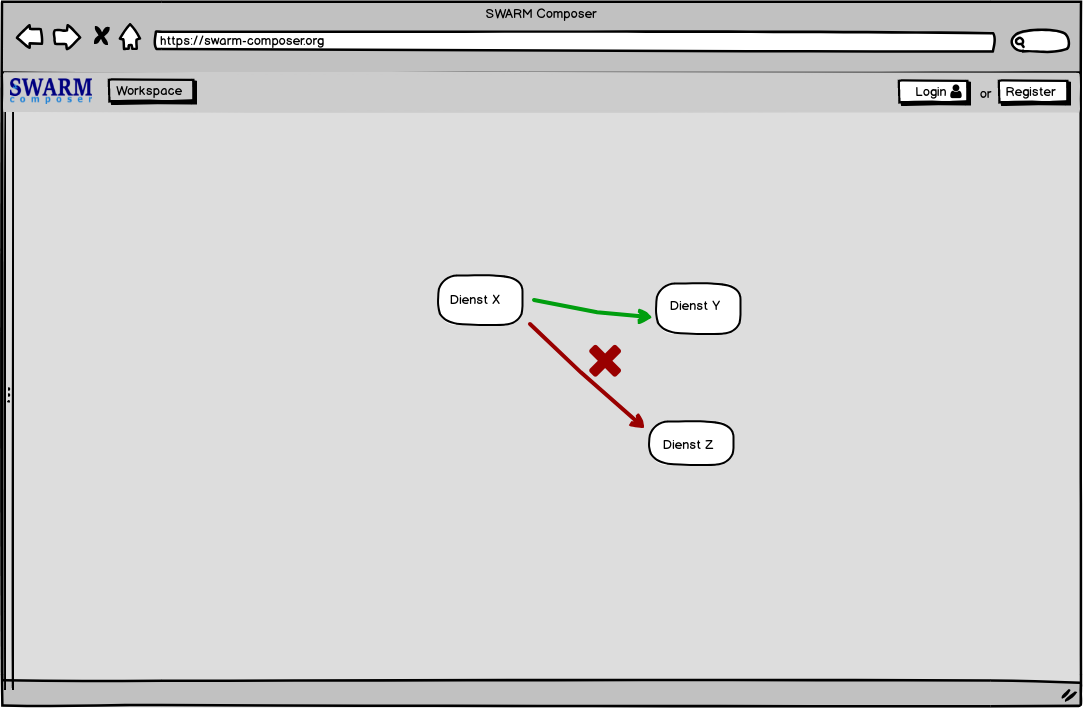
\includegraphics[width=\textwidth]{img/nichtangemeldet}
	\caption{
          Nicht angemeldete Nutzende können Kompositionen anschauen, jedoch nicht bearbeiten
        }
	\label{fig:nichtangemeldet}
\end{figure}

\begin{figure}[h]
	\centering
	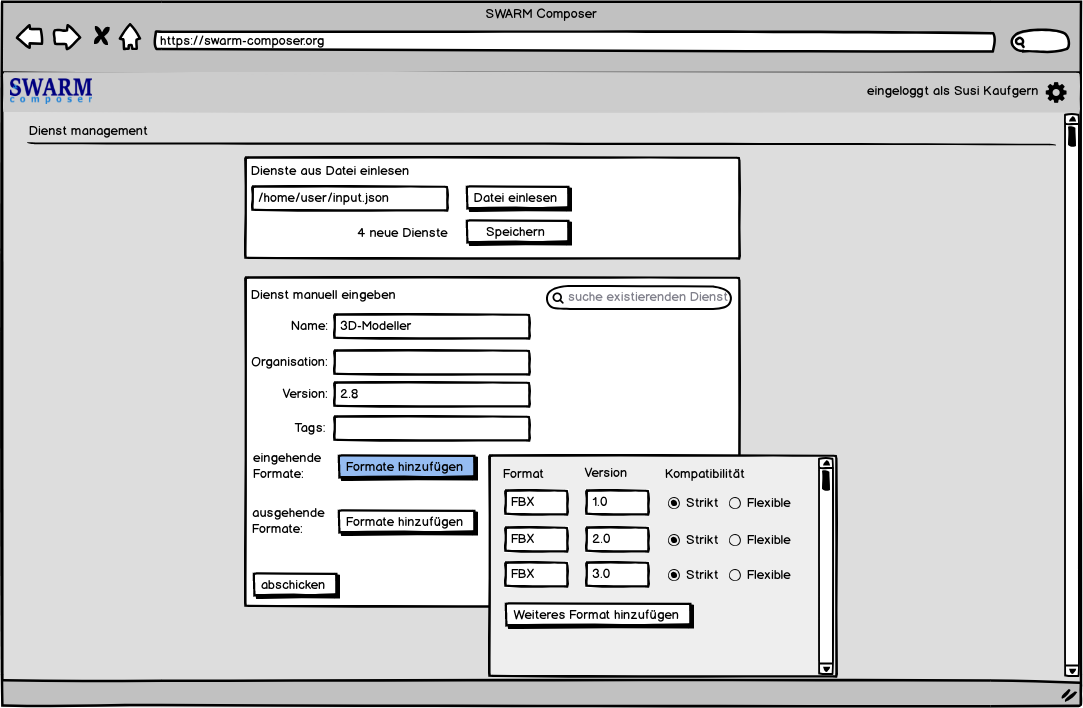
\includegraphics[width=\textwidth]{img/admin}
	\caption{
            Hier kann einE AdministratorIn neue Dienste in das System einpflegen.
            Es gibt die Wahl mehrere Dienste aus einer JSON Datei einzulesen
            oder einen neuen manuell einzupflegen. Mit dem Suchfeld kann nach Diensten
            im System gesucht werden und über die gleiche Maske verändert werden.
        }
	\label{fig:admin}
\end{figure}